\documentclass[12pt, letterpaper]{report}
\usepackage[letterpaper]{geometry}
\usepackage{hyperref}
\usepackage{graphicx}
\usepackage[english, french]{babel}
\usepackage[T1]{fontenc}
\usepackage{minted}

\usemintedstyle{vs}
\graphicspath{{./images/}}
\setminted{
  fontsize=\small, 
  breaklines=true, 
  breakanywhere=true, 
  frame=single, 
  numbers=left, 
  numbersep=5pt, 
  highlightcolor={red!20}, 
  fontfamily=consolas
}
\widowpenalties 1 10000
\raggedbottom


\begin{document}
\title{Rapport TP4 LOG3000}
\author{Stefan Cotargasanu, Faneva Rakotoarivony}
\date{\today}

\begin{center}
	\thispagestyle{empty}
	\vspace*{\stretch{1}}
	
\includegraphics[width=10cm, height=4cm]{logo-polymtl.png}\\ 
	\textbf{LOG3000 - Processus du génie logiciel} \\
	\vspace*{\stretch{1}}
	Hiver 2024 \\ 
	\vspace*{\stretch{1}}
	TP No. 4 \\ 
	\vspace*{\stretch{1}}
	2137443 - Stefan Cotargasanu \\
	2131367 - Faneva Rakotoarivony \\
	\vspace*{\stretch{1}}
	Soumis à : Patrick Loic Foalem \\
	\vspace*{\stretch{1}}
	\vspace*{\stretch{1}}
	\today
\end{center}
\pagebreak

\textbf{4.1 -  Questions d'analyse sur la section 3.1}

\textbf{1.} Expliquez avec vos propres mots ce que fait la commande \mintinline{bash}{pull alpine}. \\
La commande \mintinline{bash}{pull alpine} récupère l'image dans le registre Docker Hub et la télécharge sur la machine locale.
\newline 

\textbf{2.} Expliquez avec vos propres mots ce qui se passe derrière l'écran lorsque vous exécutez la commande \mintinline{bash}{docker run}. \\
Lorsque l'on exécute la commande \mintinline{bash}{docker run}, un conteneur lié à l'image spécifié est créé et exécuté.
\newline

\textbf{3.} Expliquez avec vos propres mots ce qui se passe derrière l'écran lorsque vous exécutez la commande \mintinline{bash}{docker run alpine echo "hello from alpine"}. S'agit-il d'une sortie de Docker ou de Linux Alpine? \\
Lorsque cette commande est exécutée, un conteneur basé sur l'image alpine est créé et lancé, dans ce conteneur la commande echo est exécutée. La sortie est celle de Alpine Linux, car la commande echo est exécutée dans le conteneur. Cette sortie est redirigée par Docker au \mintinline{bash}{stdout}.
\newline

\textbf{4.} Quelle est la différence entre une image et un conteneur? \\
La différence est qu'une image est la source d'un conteneur, un conteneur n'existe que lorsque l'image est exécutée. Une image est exécutable, lorsqu'elle est exécutée, elle créé un conteneur basé sur cette image. 
\newline

\textbf{5.} Quels sont les avantages d'un conteneur par rapport à une machine virtuelle? \\
L'avantage d'un conteneur Docker comparé à une machine virtuelle se base sur le fait que les conteneurs partagent le même noyau que la machine hôte, ce qui permet de réduire leur taille ainsi que le temps de démarrage. En comparaison, une machine virtuelle doit avoir un kernel complet. 
\newline

\textbf{4.2 Questions d'analyse de la section 3.2}

\textbf{6.} Expliquez avec vos propres mots chaque paramètre utilisé à l'étape 4 de la section 3.2
La commande lancée à l'étape 4 de la section 3.2 est \mintinline{bash}{docker run --name static-site -e AUTHOR="faneva_stefan" -d -P dockersamples/static-site}.
Nous commençons donc par \textbf{docker run} qui permet de lancer un conteneur basé sur l'image \textbf{dockersamples/static-site}. En suite, nous avons les différentes 
options utilisées:
\begin{itemize}
	\item \textbf{--name static-site} : permet de donner un nom au conteneur, dans ce cas \textbf{static-site}.
	\item \textbf{-e AUTHOR="faneva\_stefan"} : permet de définir une variable d'environnement \textbf{AUTHOR} avec la valeur \textbf{faneva\_stefan}.
	\item \textbf{-d} : permet de lancer le conteneur en mode détaché, c'est-à-dire que la console n'est pas bloquée par le process.
	\item \textbf{-P} : permet de publier tous les ports exposés par le conteneur sur des ports aléatoires de la machine hôte.
\end{itemize}
\   \\
\newline

\textbf{4.3 Questions d'analyse sur la section 3.3}\\

\textbf{7.} Expliquez la sortie de la commande \mintinline{bash}{docker} images. Comment obtenir une version spécifique d'une image?\\
La sortie de la commande \mintinline{bash}{docker images} est une liste des images disponibles localement. Pour obtenir une version spécifique d'une image, il suffit de spécifier le nom de l'image suivi de la version désirée. Par exemple, pour obtenir la version 1.0 de l'image alpine, il suffit de lancer la commande \mintinline{bash}{docker pull alpine:1.0}. Ou sinon si la question demandait comment avoir les informations sur une image spécifique, il est possible de lancer la commande \mintinline{bash}{docker images <image>:<version>}.
\newline

\textbf{8.} Expliquez avec vos propres mots la différence entre base images et child images.\\
Les images Docker sont composées de plusieurs layers. L'image de base est la première image utilisée, celle mentionnée dans le \textbf{FROM}. les child images sont des images qui sont basées sur cette image mais avec des layers supplémentaires. 
\newline

\textbf{9.} Expliquez avec vos propres mots la différence entre official images et user images.\\
Les official images sont des images prédéfinies, mises en places et maintenues par certains organismes (Docker, Canonical, RedHat, etc...) et qui sont disponibles à tous dans le registry Docker Hub. Les user images sont des images créées par des utilisateurs. 
\newline

\textbf{10.} Expliquez avec vos propres mots ce qu'est un Dockerfile.\\
Un Dockerfile est un fichier contenant une série de commande permettant au Docker Builder de créér une image. 
\newline

\textbf{11.} Expliquez chaque ligne du Dockerfile créé à l'étape 5 de la section 3.3.\\
\begin{itemize}
	\item \textbf{FROM alpine:3.5} : spécifie l'image de base, dans ce cas l'image alpine version 3.5. \\
	\item \textbf{RUN apk add --update py2-pip} : installe le paquet py2-pip, qui est un gestionnaire de paquet pour Python. \\
	\item \textbf{COPY requirements.txt /usr/src/app/} : Copie le fichier requirements.txt dans le répertoire /usr/src/app/ du conteneur. \\
	\item \textbf{RUN pip install --no-cache-dir -r /usr/src/app/requirements.txt} : Installe les dépendances spécifiées dans le fichier requirements.txt. \\
	\item \textbf{COPY app.py /usr/src/app/} : Copie le script app.py dans le répertoire /usr/src/app/ du conteneur. \\
	\item \textbf{COPY templates/index.html /usr/src/app/templates/} : Copie le fichier index.html dans le répertoire /usr/src/app/templates/ du conteneur.' \\
	\item \textbf{EXPOSE 5000} : Expose le port 5000 du conteneur. \\
	\item \textbf{CMD ["python", "/usr/src/app/app.py"]} : Définit le point d'entrée du conteneur comme étant le script app.py défini plus tôt.  \\
\end{itemize}

\textbf{12.} Expliquez ce qui se passe lorsque vous exécutez la commande \\\mintinline{bash}{docker build -t <YOUR_USERNAME>/flask-app}.
Lorsque cette commande est lancée, le builder va exécuter chacune des commandes du Dockerfile, créant une nouvelle image. \\ Cette image est ensuite taggée avec le nom spécifié, dans ce cas \textbf{<YOUR\_USERNAME>/flask-app}.\\
\newline

\textbf{13.} Décrivez chaque ligne du Dockerfile que vous avez créé. Ajoutez des captures d'écran et la sortie des commandes pour appuyer votre explication. Ajoutez également une image de votre navigateur montrant l'URL et le site Web en cours d'exécution. N'oubliez pas de soumettre le code source que vous avez développé\\
Le Dockerfile que nous avons utilisé se trouve en annexe. Ligne par ligne, voici ce qu'il fait : \\
\textbf{FROM ubuntu:22.04} : spécifie l'image de base, dans ce cas l'image ubuntu version 22.04. \\
\textbf{RUN apt-get update \&\& apt install -y python3 python3-pip}: Mets à jour les repos apt et install python ainsi que pip. \\
\textbf{COPY requirements.txt /usr/src/app}: Copie le fichier requirements.txt dans le dossier /usr/src/app/ \\
\textbf{RUN pip install --no-cache-dir -r /usr/src/app/requirements.txt}: Installe les dépendances spécifiées dans le fichier requirements.txt. \\
\textbf{COPY app.py /usr/src/app/}: Copie le script app.py de l'application dans le conteneur. \\ 
\textbf{COPY templates/index.html /usr/src/app/templates/}: Copie le template html dans le dossier /usr/src/app/templates/ \\
\textbf{EXPOSE 5000}: Expose le port 5000 du conteneur. \\
\textbf{CMD ["python3", "-m", "flask", "-A", "/usr/src/app/app.py", "run", "--host=0.0.0.0"]}: Définit le point d'entrée du conteneur comme étant le script app.py défini plus tôt en utilisant Flask. \\
\newline

Voici des captures d'écran: \\
\begin{center}
	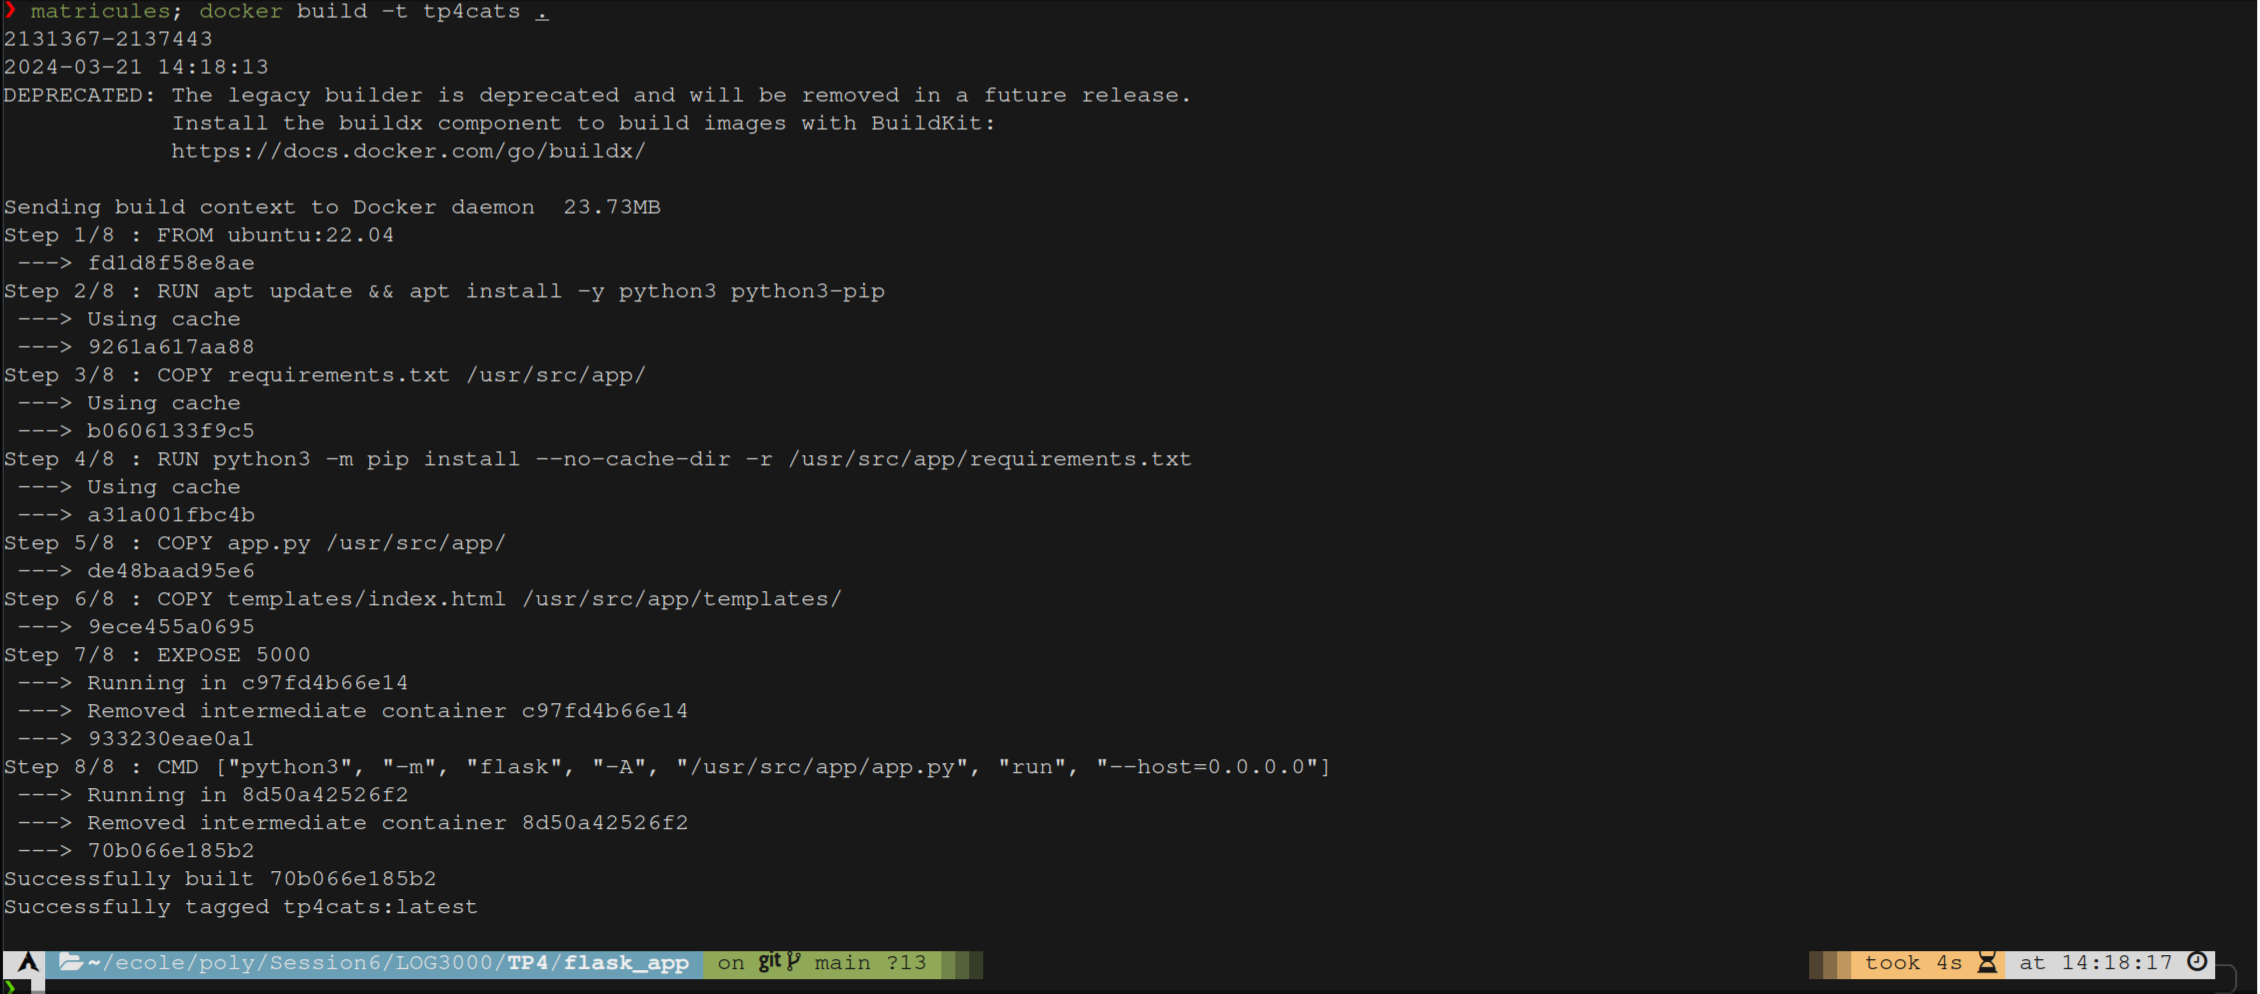
\includegraphics[scale=0.25]{4.1-build.png} \\
	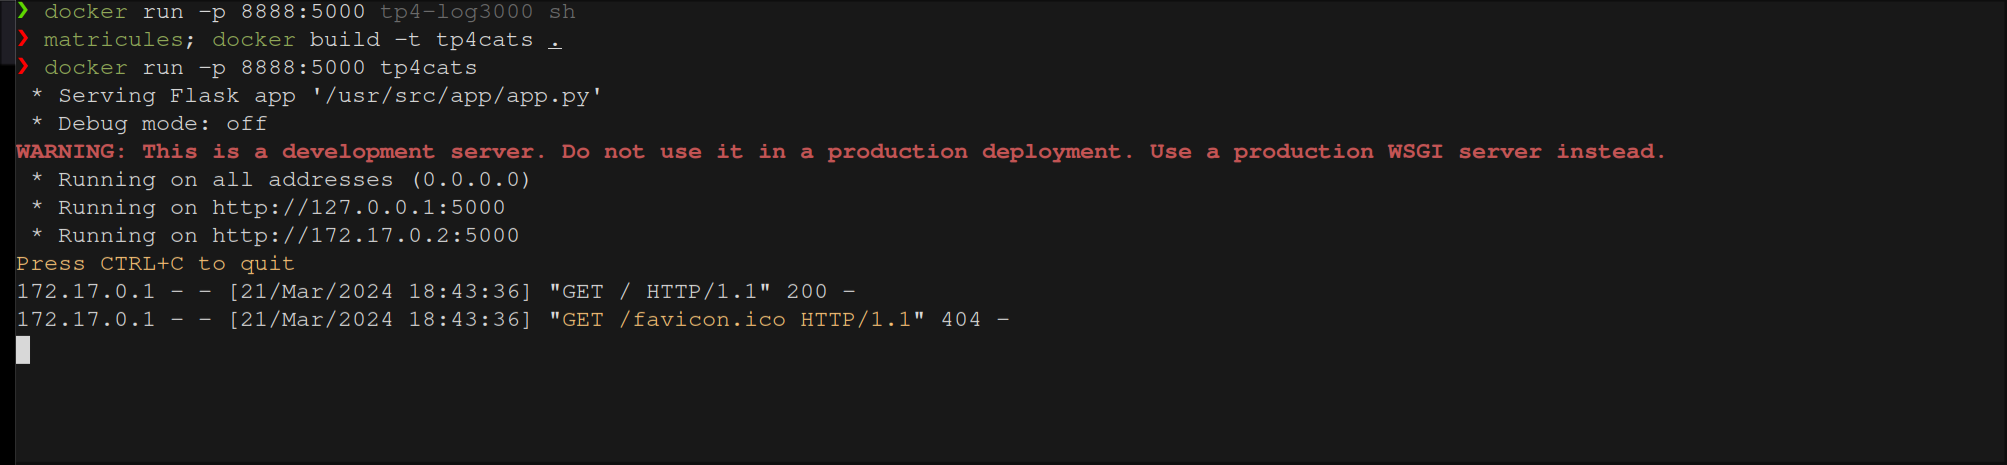
\includegraphics[scale=0.25]{4.1-run.png} \\
	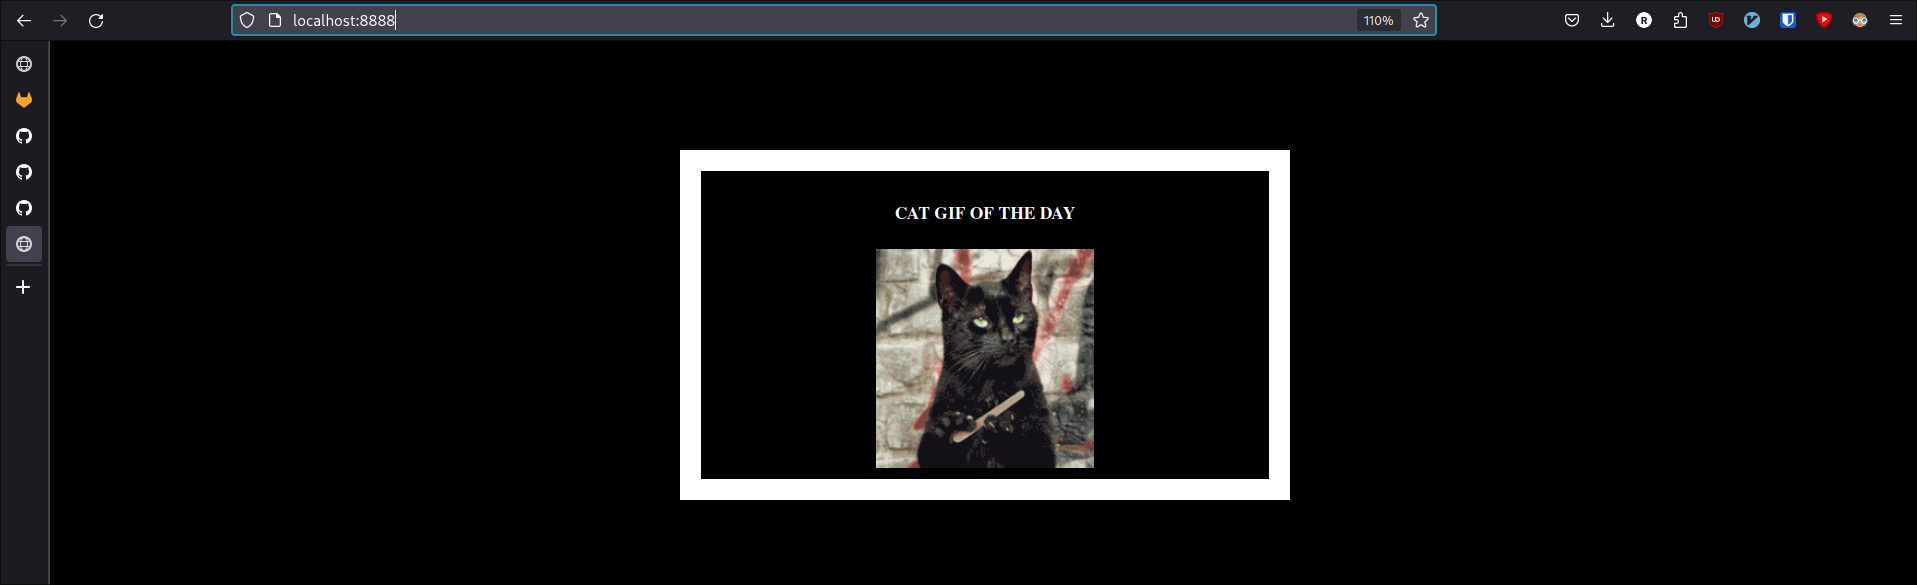
\includegraphics[scale=0.25]{4.1-app.png} \\
\end{center}

\textbf{4.4 Questions d'analyse sur la section 3.4}\\
Voici le Dockerfile que nous avons mis en place: \\
\begin{minted}{Dockerfile}
	FROM nginx:stable-alpine3.17
	
	COPY ./index.html /usr/share/nginx/html/index.html
	COPY ./animation.js /usr/share/nginx/html/animation.js  
\end{minted}
Nous nous basons sur une image de nginx qui se base sur la distribution linux d'Alpine. 
Ensuite, nous copions les fichiers index.html et animation.js dans le dossier /usr/share/nginx/html/ du conteneur. Cette page index est directement exposée par nginx.

Voici quelques captures d'écran de la création et du déploiement de l'application : \\ 
\begin{center}
	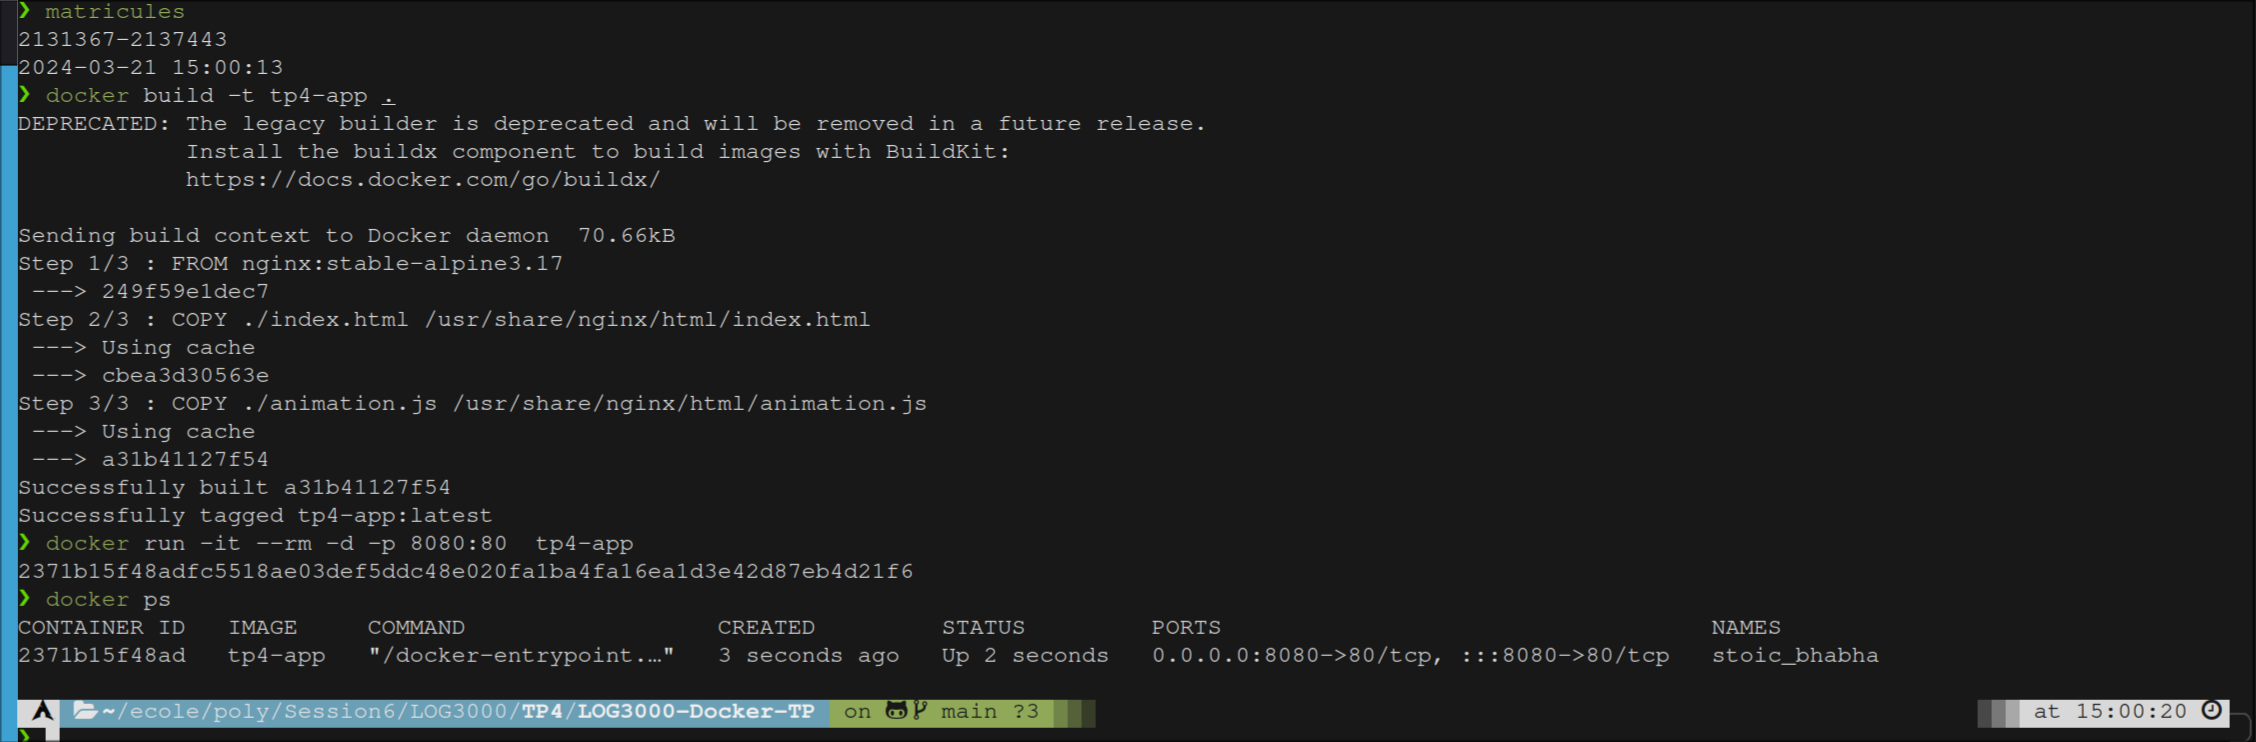
\includegraphics[scale=0.25]{4.4-all.png} \\
	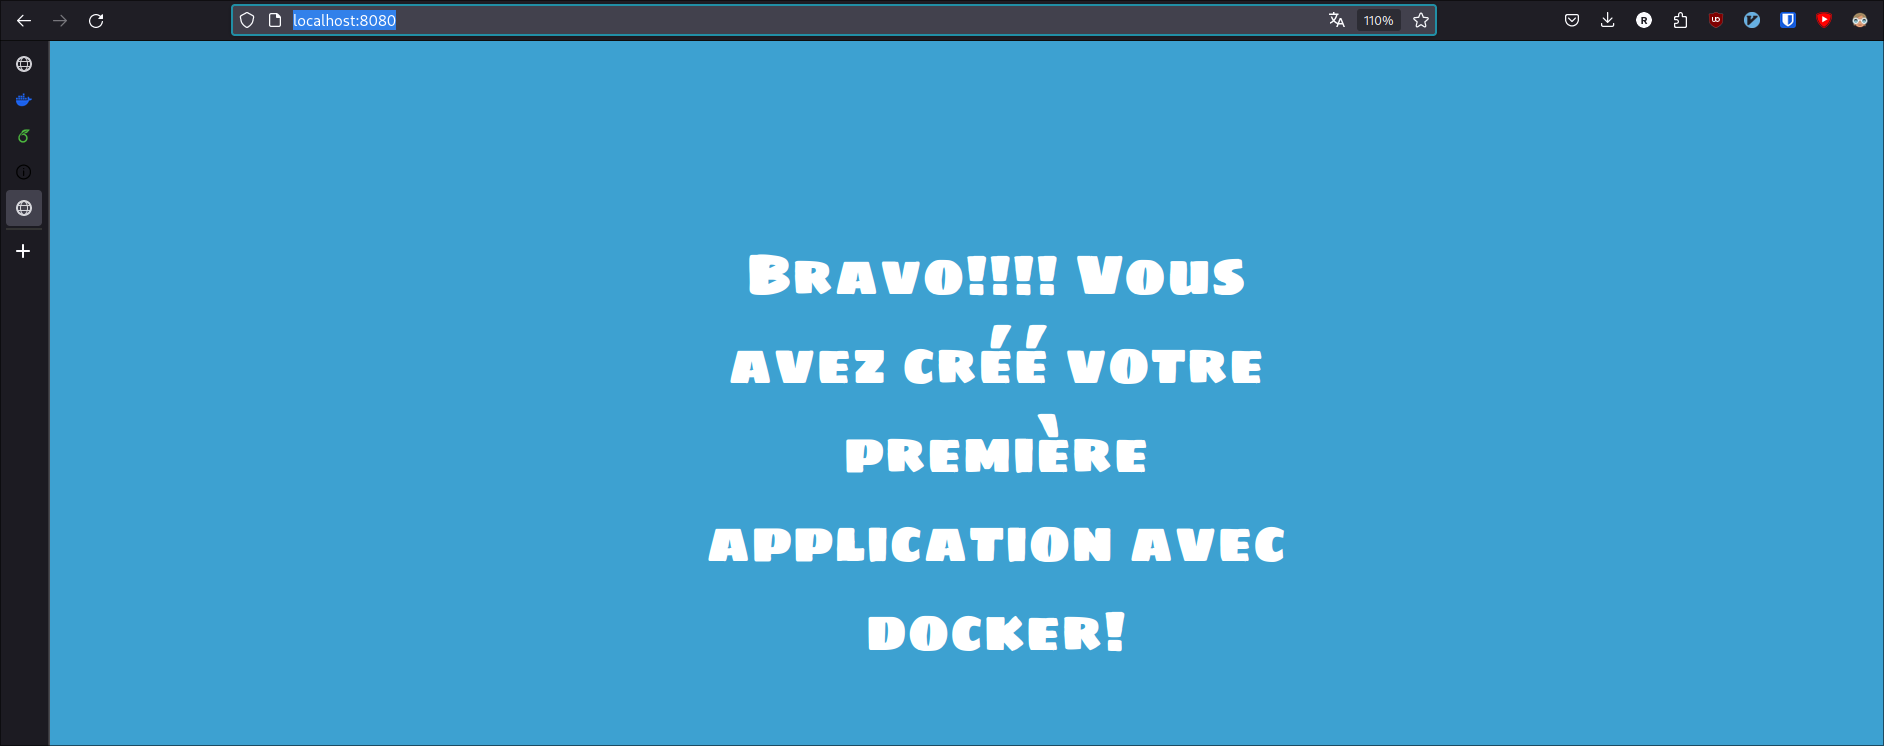
\includegraphics[scale=0.25]{4.4-app.png} \\
\end{center}
\newpage

\textbf{4.5 Question de rétroaction}\\
Nous travaillons à l’amélioration continue des travaux pratiques de LOG3000. Cette question peut être répondue très brièvement.\\
\textbf{1.} Combien de temps avez-vous passé au travail pratique, en heures-personnes, en sachant que deux personnes travaillant pendant trois heures correspondent à six heures-personnes. Est-ce que l'effort demandé pour ce laboratoire est adéquat ?\\
Nous avons passé environ 3 heures-personnes pour ce laboratoire. La partie faire le laboratoire était simple, la partie la plus longue était apprendre à utiliser \LaTeX pour la rédaction du rapport. L'effort est adéquat, le sujet est très cool. Il pourrait être pertinent d'aborder docker-compose qui est plus complet pour des applications avec plusieurs conteneurs ! 
On est un peu parti hors-sujet pour la section 4.3 mais ça reste pertinent. 
\newline

\textbf{2.} Quelles difficultés avez-vous rencontré lors de ce laboratoire?\\
Surtout \LaTeX.
\newline
\newline
Vous pourrez trouver tout le dossier source de ce TP sur le repo gitub suivant : \url{https://github.com/Fanevark/faneva_stfn_docker_tp}.


\newpage
\appendix 
\section{Dockerfile 4.3}
\begin{minted}{Dockerfile}
	FROM ubuntu:22.04
	RUN apt update && apt install -y python3 python3-pip
	COPY requirements.txt /usr/src/app/
	RUN python3 -m pip install --no-cache-dir -r /usr/src/app/requirements.txt
	COPY app.py /usr/src/app/
	COPY templates/index.html /usr/src/app/templates/
	EXPOSE 5000
	CMD ["python3", "-m", "flask", "-A", "/usr/src/app/app.py", "run", "--host=0.0.0.0"]  
\end{minted}

\newpage
\section{Flask App 4.3}
\begin{minted}{python} 
	from flask import Flask, render_template
	import random
	app = Flask(__name__)
	
	# list of cat images
	images = [
		"https://media.giphy.com/media/BzyTuYCmvSORqs1ABM/giphy.gif",
		"https://media.giphy.com/media/xUPGcyi4YxcZp8dWZq/giphy.gif",
		"https://media.giphy.com/media/1iu8uG2cjYFZS6wTxv/giphy.gif",
		"https://media.giphy.com/media/mlvseq9yvZhba/giphy.gif",
		"https://media.giphy.com/media/lJNoBCvQYp7nq/giphy.gif"
	]
	
	@app.route('/')
	def index():
		url = random.choice(images)
		return render_template('index.html', url=url)
	
	if __name__ == " main ":
		app.run(host="0.0.0.0")
\end{minted}

\end{document}
